\documentclass[10pt]{article}
\usepackage[polish]{babel}
\usepackage[utf8]{inputenc}
\usepackage[T1]{fontenc}
\usepackage{graphicx}
\usepackage[export]{adjustbox}
\graphicspath{ {./images/} }
\usepackage{amsmath}
\usepackage{amsfonts}
\usepackage{amssymb}
\usepackage[version=4]{mhchem}
\usepackage{stmaryrd}

\title{GIMNAZJUM }

\author{}
\date{}


\begin{document}
\maketitle
\begin{enumerate}
  \item Wyznacz sumę miar siedmiu kątów zaznaczonych na poniższym rysunku (w stopniach).
  \item Po przepłynięciu dwóch kilometrów rzeką pod prąd pływak napotkał płynącą z prądem butelkę. Płynął jeszcze przez pół godziny, zawrócił i dogonił butelkę dokładnie w tym momencie, w którym\\
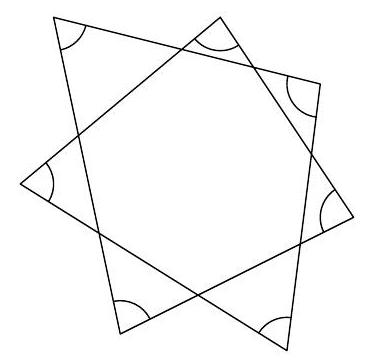
\includegraphics[max width=\textwidth, center]{2024_11_21_7354292898531eb5c521g-1}\\
dotarł do punktu wyjścia. Jaka jest prędkość wody w rzece? Zakładamy, że zarówno pływak jak i rzeka płyną ze stałą prędkością.
  \item Każdy punkt płaszczyzny pomalowano na jeden z dwóch kolorów, przy czym istnieją punkty różnych kolorów. Rozstrzygnij, czy zawsze znajdzie się trójkąt równoboczny o wierzchołkach tego samego koloru.
\end{enumerate}

\section*{LICEUM}
\begin{enumerate}
  \item Znajdź największą liczbę pięciocyfrowa składającą się z niezerowych cyfr, która ma poniższe własności:
\end{enumerate}

\begin{itemize}
  \item pierwsze trzy cyfry tworzą liczbę, która jest 9 razy większa od liczby utworzonej przez dwie ostatnie cyfry,
  \item trzy ostatnie cyfry tworzą liczbę, która jest 7 razy większa od liczby utworzonej przez pierwsze dwie cyfry.
\end{itemize}

\begin{enumerate}
  \setcounter{enumi}{1}
  \item Rozwiąż równanie
\end{enumerate}

\[
x^{x \sqrt{x}}=(x \sqrt{x})^{x}
\]

\begin{enumerate}
  \setcounter{enumi}{2}
  \item Każdy punkt płaszczyzny pomalowano na jeden z dwóch kolorów. Rozstrzygnij, czy zawsze znajdziemy takie trzy parami różne punkty jednego koloru, aby jeden z nich był środkiem odcinka, którego końcami są dwa pozostałe.
\end{enumerate}

\end{document}